Given $\Pi_{MAC}$ = (Gen, Enc, Ver)

\begin{center}
    $ t \leftarrow c = Enc(k,m) $ 
\end{center}

To prove if this construction is secure or not, the reduction is as in Figure \ref{Reduction}

\begin{figure}[h]
    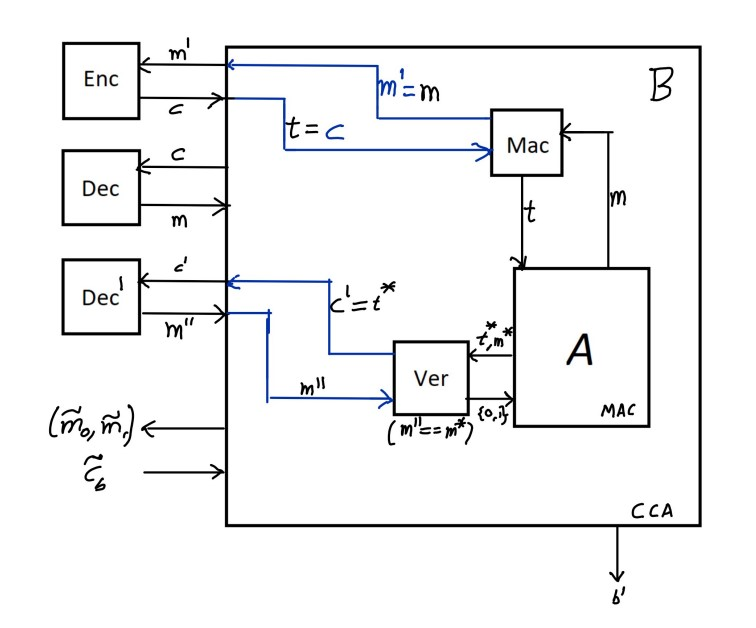
\includegraphics[width=\textwidth,height=\textheight,keepaspectratio]{8-1.jpg}
    \caption{Proof by Reduction}
    \label[figure]{Reduction}
    \centering
\end{figure}

First lets assume the contradiction that the construction is not secure MAC. That is probablity of forging
this construction $\Pi_{MAC}$ is a non negligible function. i.e.,

\begin{center}
    $Pr[MacForge_{A,\Pi_{MAC}} = 1] \leq \epsilon(\lambda)$
\end{center}
where $\epsilon(\lambda)$ is a non negligible function.\\


That implies there exists an adversary, A, able to generate a new message and tag pair $(m^*, t^*)$
such that $m^* \notin Q $, and $Ver_k(m^*, t^*) == 1$ with a probablity $\epsilon(\lambda)$. 
% As per the reduction, Ver uses the Dec by comparing $m^*$ with the message from Dec as shown in the Figure \ref*{Reduction}. 
\newline


That implies
\begin{align}
    Pr[ PrivK_{A,\Pi}(\lambda) = 1  \wedge \overline{ValidQuery}]  \leq \epsilon(\lambda)
    \label{eq1}
\end{align}
where $\epsilon(\lambda)$ is a non negligible function.\\



But given that $\Pi$ is a CCA secure enryption scheme. And for CCA,
\begin{align}
    Pr[ PrivK_{A,\Pi}^{CCA}(\lambda) = 1  \wedge \overline{ValidQuery}]  \leq 1/2 + neg(\lambda)
    \label{eq2}
\end{align}


Equation (\ref*{eq1}) and (\ref*{eq2}) are contradecting to each other. Thus our assumption is
false and this construction is secure.


